\documentclass[11pt,a4paper]{article}
\newcommand{\doclang}{pt}
\newcommand{\doctitle}{História das Matrículas Portuguesas}
\usepackage{etoolbox}
% Shared preamble for historia-pt.tex and history-en.tex (XeTeX via Tectonic).
% The wrapper defines \doclang (pt|en) before % Shared preamble for historia-pt.tex and history-en.tex (XeTeX via Tectonic).
% The wrapper defines \doclang (pt|en) before % Shared preamble for historia-pt.tex and history-en.tex (XeTeX via Tectonic).
% The wrapper defines \doclang (pt|en) before \input{preamble}.
% Standard article styling throughout; only the cover has its own look.
\usepackage{fontspec}
\ifdefstring{\doclang}{pt}{\usepackage[portuguese]{babel}}{\usepackage[british]{babel}}

\usepackage{graphicx}
\graphicspath{{figures/}}
\usepackage{booktabs, longtable, array, multicol, needspace}
\usepackage[hidelinks]{hyperref}
\usepackage{xurl}

% --- Cover only ---------------------------------------------------------------
\usepackage{xcolor}
\definecolor{accent}{HTML}{1F5FB4}
\newfontfamily\coverfont{texgyreheros}[
  Extension = .otf,
  UprightFont = *-regular,
  BoldFont = *-bold,
]

% --- Macros -------------------------------------------------------------------
% A plate number, kept on one line.
\newcommand{\plate}[1]{\mbox{\textbf{#1}}}
% A code in the annex tables.
\newcommand{\code}[1]{\mbox{\texttt{#1}}}
% Marks an annex table entry the sources do not confirm.
\newcommand{\unverified}{\textsuperscript{†}}
% Small photo inside an annex table row.
\newcommand{\tablephoto}[1]{\raisebox{-0.35\height}{\includegraphics[height=0.75cm]{#1}}}
% \platefig[width]{file}{caption}
\newcommand{\platefig}[3][0.45\linewidth]{%
  \begin{figure}[htbp]\centering\includegraphics[width=#1]{#2}\caption{#3}\end{figure}}
% Two plates side by side: \platepair{file1}{caption1}{file2}{caption2}
\newcommand{\platepair}[4]{%
  \begin{figure}[htbp]\centering
  \begin{minipage}[b]{0.46\linewidth}\centering\includegraphics[width=\linewidth,height=3.2cm,keepaspectratio]{#1}\caption{#2}\end{minipage}\hfill
  \begin{minipage}[b]{0.46\linewidth}\centering\includegraphics[width=\linewidth,height=3.2cm,keepaspectratio]{#3}\caption{#4}\end{minipage}
  \end{figure}}

% Lets lines with long unbreakable plate numbers stretch instead of overflowing.
\setlength{\emergencystretch}{3em}

\newcommand{\gen}[1]{\input{generated/\doclang/#1}}
.
% Standard article styling throughout; only the cover has its own look.
\usepackage{fontspec}
\ifdefstring{\doclang}{pt}{\usepackage[portuguese]{babel}}{\usepackage[british]{babel}}

\usepackage{graphicx}
\graphicspath{{figures/}}
\usepackage{booktabs, longtable, array, multicol, needspace}
\usepackage[hidelinks]{hyperref}
\usepackage{xurl}

% --- Cover only ---------------------------------------------------------------
\usepackage{xcolor}
\definecolor{accent}{HTML}{1F5FB4}
\newfontfamily\coverfont{texgyreheros}[
  Extension = .otf,
  UprightFont = *-regular,
  BoldFont = *-bold,
]

% --- Macros -------------------------------------------------------------------
% A plate number, kept on one line.
\newcommand{\plate}[1]{\mbox{\textbf{#1}}}
% A code in the annex tables.
\newcommand{\code}[1]{\mbox{\texttt{#1}}}
% Marks an annex table entry the sources do not confirm.
\newcommand{\unverified}{\textsuperscript{†}}
% Small photo inside an annex table row.
\newcommand{\tablephoto}[1]{\raisebox{-0.35\height}{\includegraphics[height=0.75cm]{#1}}}
% \platefig[width]{file}{caption}
\newcommand{\platefig}[3][0.45\linewidth]{%
  \begin{figure}[htbp]\centering\includegraphics[width=#1]{#2}\caption{#3}\end{figure}}
% Two plates side by side: \platepair{file1}{caption1}{file2}{caption2}
\newcommand{\platepair}[4]{%
  \begin{figure}[htbp]\centering
  \begin{minipage}[b]{0.46\linewidth}\centering\includegraphics[width=\linewidth,height=3.2cm,keepaspectratio]{#1}\caption{#2}\end{minipage}\hfill
  \begin{minipage}[b]{0.46\linewidth}\centering\includegraphics[width=\linewidth,height=3.2cm,keepaspectratio]{#3}\caption{#4}\end{minipage}
  \end{figure}}

% Lets lines with long unbreakable plate numbers stretch instead of overflowing.
\setlength{\emergencystretch}{3em}

\newcommand{\gen}[1]{\input{generated/\doclang/#1}}
.
% Standard article styling throughout; only the cover has its own look.
\usepackage{fontspec}
\ifdefstring{\doclang}{pt}{\usepackage[portuguese]{babel}}{\usepackage[british]{babel}}

\usepackage{graphicx}
\graphicspath{{figures/}}
\usepackage{booktabs, longtable, array, multicol, needspace}
\usepackage[hidelinks]{hyperref}
\usepackage{xurl}

% --- Cover only ---------------------------------------------------------------
\usepackage{xcolor}
\definecolor{accent}{HTML}{1F5FB4}
\newfontfamily\coverfont{texgyreheros}[
  Extension = .otf,
  UprightFont = *-regular,
  BoldFont = *-bold,
]

% --- Macros -------------------------------------------------------------------
% A plate number, kept on one line.
\newcommand{\plate}[1]{\mbox{\textbf{#1}}}
% A code in the annex tables.
\newcommand{\code}[1]{\mbox{\texttt{#1}}}
% Marks an annex table entry the sources do not confirm.
\newcommand{\unverified}{\textsuperscript{†}}
% Small photo inside an annex table row.
\newcommand{\tablephoto}[1]{\raisebox{-0.35\height}{\includegraphics[height=0.75cm]{#1}}}
% \platefig[width]{file}{caption}
\newcommand{\platefig}[3][0.45\linewidth]{%
  \begin{figure}[htbp]\centering\includegraphics[width=#1]{#2}\caption{#3}\end{figure}}
% Two plates side by side: \platepair{file1}{caption1}{file2}{caption2}
\newcommand{\platepair}[4]{%
  \begin{figure}[htbp]\centering
  \begin{minipage}[b]{0.46\linewidth}\centering\includegraphics[width=\linewidth,height=3.2cm,keepaspectratio]{#1}\caption{#2}\end{minipage}\hfill
  \begin{minipage}[b]{0.46\linewidth}\centering\includegraphics[width=\linewidth,height=3.2cm,keepaspectratio]{#3}\caption{#4}\end{minipage}
  \end{figure}}

% Lets lines with long unbreakable plate numbers stretch instead of overflowing.
\setlength{\emergencystretch}{3em}

\newcommand{\gen}[1]{\input{generated/\doclang/#1}}


\begin{document}
\pagenumbering{alph}
\begin{titlepage}
  \coverfont
  \centering
  {\fontsize{34}{40}\selectfont\bfseries\color{accent} História das\\ Matrículas Portuguesas\par}
  \vspace{0.8cm}
  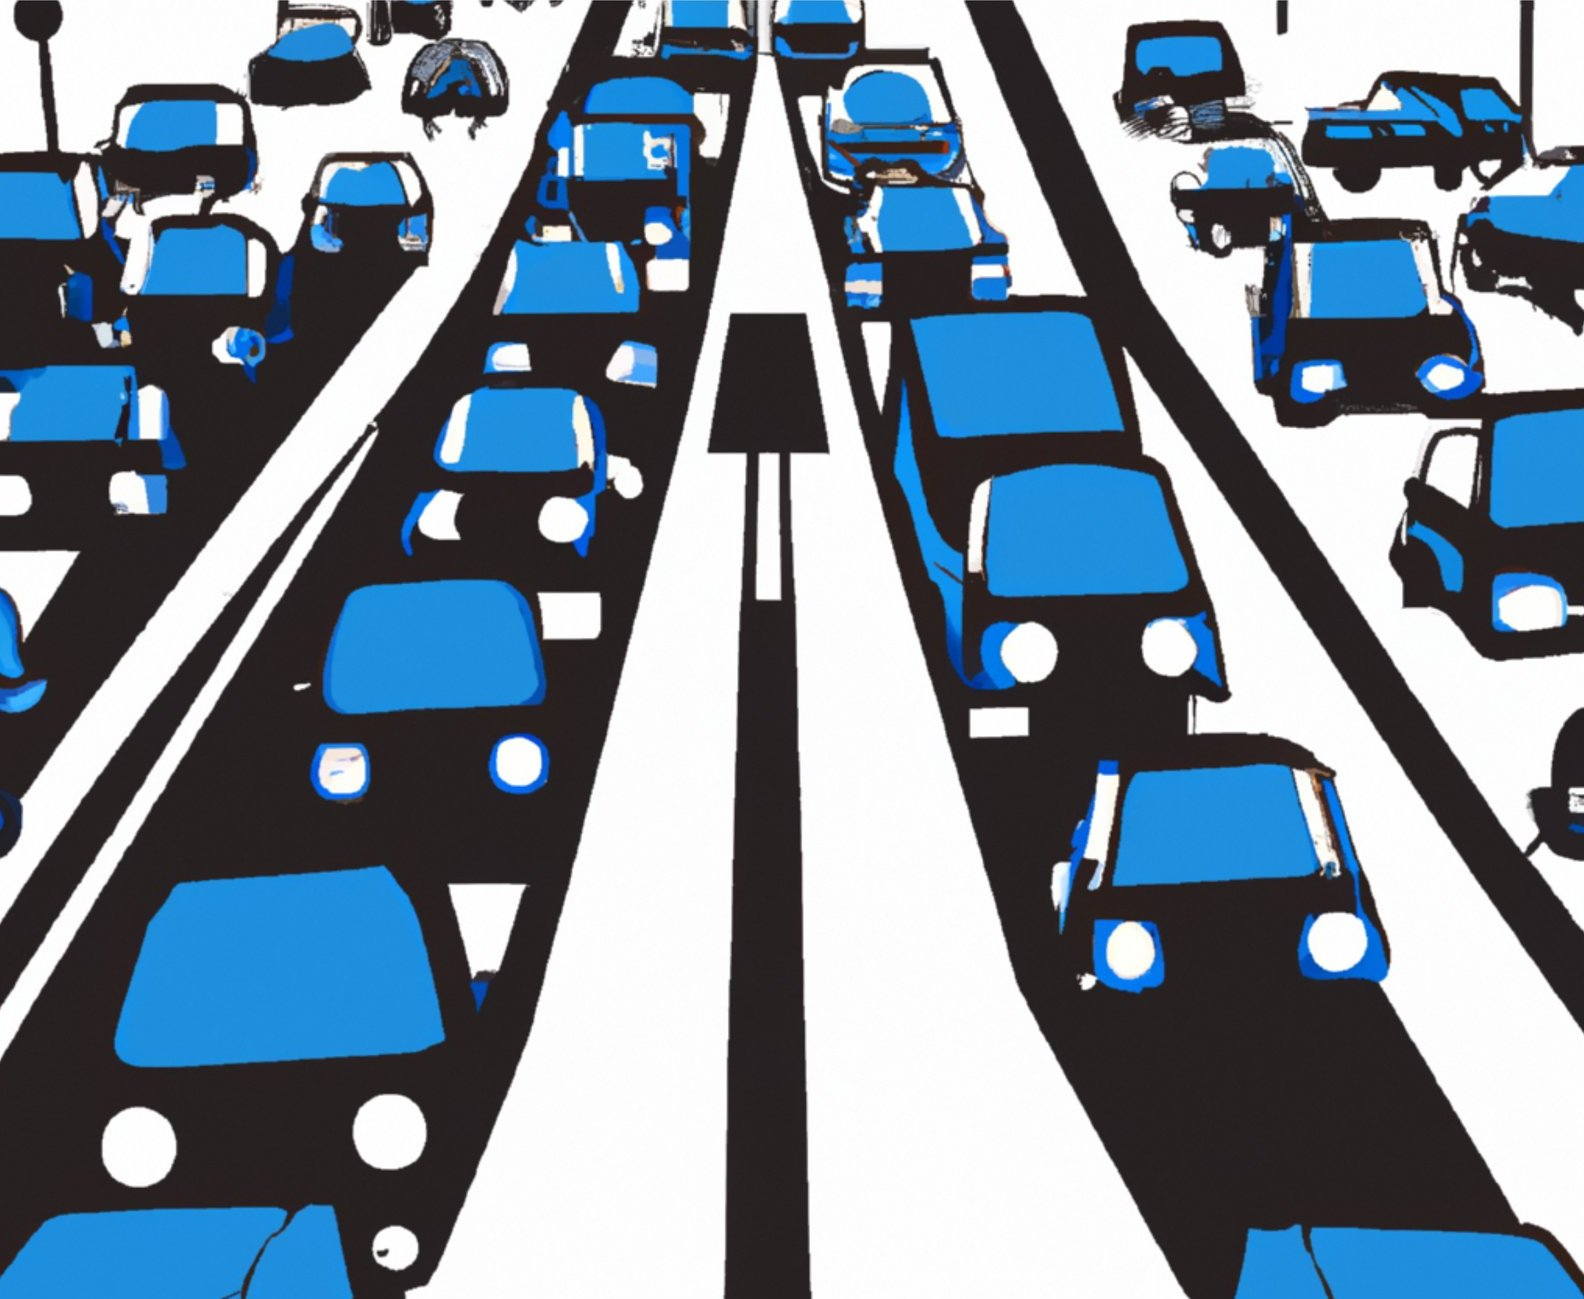
\includegraphics[width=\linewidth]{cover-illustration}
  \vspace{0.8cm}

  \begin{minipage}[t]{0.6\linewidth}
    {\large\bfseries\color{accent} Uma viagem desde a primeira licença em 1901 até ao século XXI\par}
  \end{minipage}\hfill
  \begin{minipage}[t]{0.35\linewidth}\raggedleft
    {\large\bfseries\color{accent} José Rodrigues\par}
    \vspace{0.3em}
    {\small 2023, revisto em \the\year\par}
  \end{minipage}
\end{titlepage}

\pagenumbering{arabic}
\tableofcontents
\clearpage
\section{Matrículas}

Com exceção das matrículas de época, os formatos das matrículas devem ser
utilizados de acordo com a data da matriculação em Portugal. Podem-se utilizar
matrículas de formatos mais recentes, mas não se podem utilizar formatos
anteriores, sob pena de autuação pelas autoridades.

\begin{figure}[htbp]
  \centering
  \begin{tabular}{@{}c c@{}}
    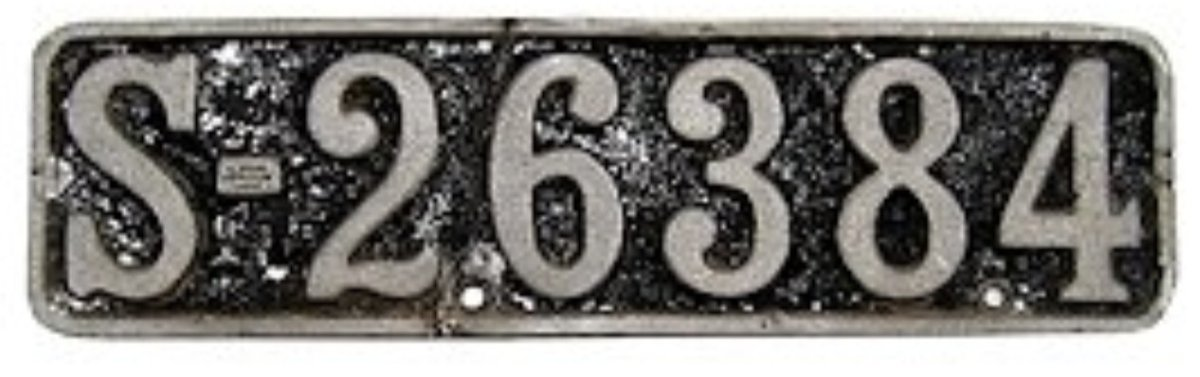
\includegraphics[height=1.3cm]{fmt-1911} & 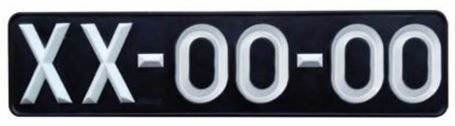
\includegraphics[height=1.3cm]{fmt-1937} \\
    \small 1911 a 31/12/1936 & \small 1/1/1937 a 31/12/1991 \\[0.6em]
    
\includegraphics[height=1.3cm]{fmt-1992} & 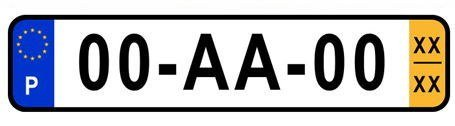
\includegraphics[height=1.3cm]{fmt-2005} \\
    \small 1/1/1992 a 31/12/1997 & \small 1/1/1998 a 2/3/2020 \\[0.6em]
    \multicolumn{2}{c}{
\includegraphics[height=1.3cm]{fmt-2020}} \\
    \multicolumn{2}{c}{\small A partir de 3/3/2020}
  \end{tabular}
  \caption{Os cinco formatos de matrícula e o período em que cada aparência foi atribuída. A edição de 2023 indicava 31/12/2019 e 1/1/2020. O Decreto-Lei n.º 2/2020
liga o novo modelo de chapa ao início da emissão do novo formato, e a primeira
matrícula \plate{AA 01 AA} foi emitida a 3 de março de 2020 (IMT).}
\end{figure}

As chapas de matrícula mais recentes seguem o modelo europeu: cor branca
refletora como base, caracteres a preto. No lado esquerdo é colocada a banda
azul (“eurobanda”) com a letra de identificação nacional: \plate{P}.

No lado direito, até à última alteração, surgia a barra amarela com a indicação
do mês e do ano do primeiro registo do veículo (por exemplo, um carro de junho
de 1997 teria indicado \plate{97/06}).

Mas se o carro foi matriculado antes de 1 de janeiro de 1998, pode usar o modelo
em vigor à data da matrícula, ou seja:
\begin{itemize}
  \item chapas pretas com caracteres brancos para os que foram matriculados até
        31 de dezembro de 1991;
  \item chapas brancas com a eurobanda azul, mas sem a barra amarela, para os
        veículos matriculados entre 1 de janeiro de 1992 e 31 de dezembro de 1997.
\end{itemize}

Os veículos antigos considerados de interesse museológico podem usar uma chapa do
modelo em vigor quando entraram em circulação. Os automóveis têm duas chapas, uma
à frente e outra atrás (Decreto-Lei n.º~54/2005, art.~7.º; ver a
secção~\ref{sec:legislacao}).

\needspace{14\baselineskip}
\gen{series}

\clearpage
\section{1901 | As primeiras matrículas portuguesas}
\subsection*{Licenças de circulação de automóveis}

As primeiras matrículas surgiram a 3 de outubro de 1901, então denominadas
“licenças de circulação de automóveis”. Nesta altura eram emitidas pelos
Governos Civis dos Distritos e apenas era obrigatória uma chapa de matrícula na
parte de trás do veículo, embora as fotografias da época mostrem que por vezes
também era colocada à frente.

As combinações eram compostas pelo nome ou pela abreviatura da sede de distrito
que atribuiu a licença e pelo número, podendo assim ver-se matrículas como
\plate{LISBOA 130} ou \plate{LXA 256}.

O decreto com essa data estabelecia a obrigatoriedade de todos os automóveis
trazerem na parte de trás uma chapa metálica com os caracteres do número da
licença e da sede de distrito onde foi concedida.

O primeiro registo automóvel em Portugal foi feito em nome de Augusto Sabido
Teixeira de Aragão, de Santiago do Cacém.

\section{1911 | Série X-000}
\subsection*{1.ª padronização do sistema de matrículas português}

Com o aumento do número de carros em Portugal, o sistema foi padronizado a
nível nacional. O país foi dividido em norte, centro e sul, com a inicial de
cada zona a anteceder os algarismos. As chapas eram pretas com caracteres
brancos, com sequências como \plate{N-000}, \plate{C-000} e \plate{S-000}, ou
\plate{N-00000}, \plate{C-00000} e \plate{S-00000}.

\platefig{fmt-1911}{Matrícula da série de 1911: \plate{S-26384}.}

\begin{itemize}
  \item Nos automóveis de aluguer era colocado um \plate{A} no final do número de
        série. Ex.: \plate{C-4569-A}.
  \item Nas matrículas provisórias acrescentavam-se as letras \plate{WW}.
        Ex.: \plate{S-1703-WW}.
  \item Os automóveis do Exército usavam a sequência \plate{MG-000}, que se
        manteve em uso até à década de 1950.
\end{itemize}

\section{1918 | Zonas de registo dos Açores e da Madeira}

Foram atribuídas aos Açores e à Madeira, respetivamente, as séries \plate{A-000}
e \plate{M-000}. Ao contrário do que aconteceu no continente, este sistema
manteve-se em vigor nas ilhas até 1962.

\section{1937 | Série XX-00-00}
\subsection*{2.ª padronização do sistema de matrículas português}

Em algumas zonas o número de série já chegava aos cinco algarismos, o que
dificultava a rápida identificação da viatura. Foi nesta altura que começaram as
combinações que conhecemos, com duas letras e dois pares de algarismos.

A 1 de janeiro de 1937 entrou em vigor o 2.º sistema nacional de matriculação de
automóveis. Manteve-se a divisão por zonas, mas agora por grupos de letras:
\begin{itemize}
  \item de \plate{AA} a \plate{LZ} para a Zona de Lisboa;
  \item de \plate{MA} a \plate{TZ} para a Zona do Porto;
  \item de \plate{UA} a \plate{ZZ} para a Zona de Coimbra (antiga zona Centro).
\end{itemize}

As chapas continuaram a ser de fundo preto com caracteres a branco, com exceção
dos veículos diplomáticos ou em importação temporária, e eram de plástico, com
os caracteres em relevo.

\platefig{1937-pg0870}{Matrícula da série de 1937: \plate{PG-08-70}, da Zona do Porto.}

Não foi autorizado o uso das letras \plate{Q} e \plate{J}, por se confundirem
respetivamente com \plate{O} e com \plate{I}, e por razões de “decência” foi
interdito o uso dos grupos de letras \plate{CU} e \plate{FD}.

Alguns grupos de letras foram sendo reservados a organizações e entidades:\footnote{Segundo a Wikipédia (\emph{Matrículas de automóveis em Portugal}); a edição de 2023 não os referia.}
\begin{itemize}
  \item \plate{MG}, \plate{ME} e \plate{MX} para o Exército, \plate{AP} para a
        Marinha, \plate{AM} para a Força Aérea e \plate{EP} para a Administração
        Civil do Estado;
  \item \plate{CD}, \plate{CC} e \plate{FM}, em caracteres vermelhos sobre fundo
        branco, para o Corpo Diplomático, o Corpo Consular e outros funcionários
        em missão diplomática (até 1985, ver mais abaixo);
  \item \plate{TA}, \plate{TB} e \plate{TC}, em caracteres brancos sobre fundo
        vermelho, para os veículos em importação temporária das zonas de Lisboa,
        Porto e Coimbra.
\end{itemize}
A Guarda Nacional Republicana e a antiga Guarda Fiscal tinham sequências
próprias, começadas respetivamente por \plate{GNR} e \plate{GF}.

\subsection{Conversão das matrículas de 1911}

Os automóveis registados pelo sistema de 1911 foram obrigados a mudar para o
novo, através da atribuição de séries específicas de acordo com a matrícula
anterior. Os quatro algarismos finais do número antigo passaram a formar os dois
pares de algarismos.

\begin{itemize}
  \item \textbf{Lisboa:} \plate{S-000} e \plate{S-0000} passaram para \plate{AA-00-00};
        \plate{S-10000} para \plate{AB-00-00}; \plate{S-20000} para \plate{AC-00-00};
        \plate{S-30000} para \plate{AD-00-00}.
        Ex.: \plate{S-12345} passou para \plate{AB-23-45}.
  \item \textbf{Porto:} \plate{N-000} e \plate{N-0000} para \plate{MM-00-00};
        \plate{N-10000} para \plate{MN-00-00}.
        Ex.: \plate{N-1234} passou para \plate{MM-12-34}.
  \item \textbf{Coimbra:} todos os veículos mudaram para a série \plate{UU-00-00}.
        Ex.: \plate{C-123} passou para \plate{UU-01-23}.
\end{itemize}

\section{1962 | Adoção do sistema de matriculação nas ilhas}

Nos Açores e na Madeira o novo sistema só foi adotado em 1962. Os Açores foram
divididos em três zonas de matriculação, correspondentes aos Distritos Autónomos
de Ponta Delgada, Angra do Heroísmo e Horta, cada um com serviços próprios de
matrícula, e a Madeira constituía apenas uma zona, correspondente ao Distrito
Autónomo do Funchal. As letras reservadas a estas zonas foram:
\begin{itemize}
  \item \plate{AN} para Angra do Heroísmo;
  \item \plate{AR} e \plate{AS} para Ponta Delgada;
  \item \plate{HO} para a Horta;
  \item \plate{MA} e \plate{MD} para o Funchal.
\end{itemize}

As letras \plate{TD}, \plate{TG}, \plate{TH} e \plate{TF}, em caracteres brancos
sobre fundo vermelho, foram reservadas para os veículos em importação temporária
de Ponta Delgada, Angra do Heroísmo, Horta e Funchal, respetivamente.

\section{Anos 70 | Novos serviços regionais}

Na década de 1970 foram sendo estabelecidos novos serviços regionais e as
respetivas zonas de matrícula, com grupos de letras reservados:
\begin{itemize}
  \item \plate{EM} e \plate{EV} para Évora;
  \item \plate{ZA} e \plate{ZB} para Braga;
  \item \plate{ZC} e \plate{ZD} para Vila Real;
  \item \plate{ZE} e \plate{ZF} para Aveiro;
  \item \plate{ZG} e \plate{ZH} para a Guarda;
  \item \plate{ZI} e \plate{ZL} para Santarém;
  \item \plate{ZM} e \plate{ZN} para Setúbal;
  \item \plate{ZO} e \plate{ZP} para Faro.
\end{itemize}

O registo de Évora era considerado central a nível regional, pelo que lhe foi
também atribuído um código para veículos em importação temporária: \plate{TE}.
Como o registo por zonas foi descontinuado pouco tempo depois, a maioria destes
grupos de letras não chegou a ser usada como identificador de zona.

Com a independência das colónias portuguesas, quem quisesse podia importar o seu
carro para Portugal. Para o efeito foram atribuídas novas matrículas com as
iniciais \plate{VZ}, \plate{ZO}, \plate{ZE} e \plate{UZ}.\footnote{A atribuição de \plate{ZE} e \plate{UZ} a estas importações está por confirmar.}
\plate{VZ} era referido com humor como “Veio Zangado”.

\section{Anos 80 | Extensão do sistema de 1937}

No princípio da década de 1980, com o esgotamento das séries reservadas a algumas
zonas, acabou-se com a separação por zonas e os veículos passaram a ser
matriculados sequencialmente a nível nacional.

Mesmo assim, a série \plate{AA-00-00} aproximava-se rapidamente do fim. Para o
adiar, foi autorizada a utilização das “famosas” combinações \plate{CU} e
\plate{FD} e das letras \plate{Q} e \plate{J}.

Em 1985 as matrículas diplomáticas passaram a ter uma sequência diferente da
normal, nos formatos \plate{000-CD000}, \plate{000-CC000} e \plate{000-FM000}, em
que o primeiro grupo de algarismos identifica o país do utilizador do veículo e
o grupo de letras o seu estatuto diplomático (ver
secção~\ref{sec:diplomaticos}).

\platefig{diplomatic-fm}{Matrícula diplomática \plate{024-FM256}.}

\section{1992 | Série 00-00-XX}
\subsection*{Nova numeração e eurobanda}

Em 1992 as chapas mudaram de aparência e de numeração. Passaram a ser usadas
placas brancas refletoras com letras pretas e uma faixa azul do lado esquerdo
(eurobanda) com a identificação da União Europeia e a inicial do país, neste caso
\plate{P}. A fonte das letras é a DIN 1451, criada pelo Instituto Alemão de
Normalização em 1931. As novas chapas eram metálicas e Portugal foi o segundo
país a adotar a eurobanda.

A numeração passou a ter as letras no fim: \plate{00-00-AA}. As duas mudanças
não foram simultâneas: a nova chapa aplica-se às matrículas a partir de
1 de janeiro de 1992, mas a numeração \plate{00-00-AA} só começou a 1 de março
(Decreto-Lei n.º~54/2005, arts.~3.º e~5.º). Nos dois primeiros meses de 1992
foram, portanto, atribuídas matrículas \plate{AA-00-00} já em chapa branca.

Na nova sequência nenhum grupo de letras foi reservado a entidades especiais. A
única exceção foram as importações de 1997 (secção~\ref{sec:importados}).

\platefig{1992-7293fq}{Matrícula da série de 1992, sem barra amarela: \plate{72-93-FQ}.}

\section{1998 | Ano e mês do primeiro registo}

Mantendo a numeração de 1992, a aparência mudou: do lado direito passou a haver
uma faixa amarela com o ano e o mês do primeiro registo do veículo.

\platefig{1998-4572xq}{\plate{45-72-XQ}, com a barra amarela de junho de 2004.}

\section{2005 | Série 00-XX-00}

Esgotadas as combinações da numeração anterior, as matrículas passaram em 2005 a
ter o formato \plate{00-XX-00}.

\platefig{2005-99sa99}{Matrícula da série de 2005: \plate{99-SA-99}.}

\section{2020 | Série XX 00 XX}

Em 2020 mudaram tanto a numeração como a aparência das matrículas, para o
sistema usado atualmente. O Decreto-Lei n.º 2/2020, de 14 de janeiro, definiu o
novo número de matrícula como “dois grupos de duas letras e um grupo central de
dois algarismos”, um formato que o Decreto-Lei n.º~54/2005 já previa para quando
se esgotasse a série \plate{00-AA-00}. Segundo o IMT, aplica-se só a veículos
novos; o dono de um veículo de uma série anterior pode pedir uma chapa sem o mês
e o ano. A primeira matrícula, \plate{AA 01 AA}, foi emitida a 3 de março
de 2020 e atribuída a um veículo elétrico; a combinação \plate{AA 00 AA} ficou
reservada pelo IMT “para memória futura”.

\platefig{2020-aa16aa}{Matrícula da série de 2020: \plate{AA 16 AA}.}

Os traços foram substituídos por espaços, porque não haveria espaço suficiente
para números de matrícula com várias letras largas. A barra amarela com o ano e
o mês da primeira matrícula foi retirada para uniformizar as chapas com as dos
restantes países da União Europeia: Portugal era o único dos 27 Estados-Membros
com esta informação, que se podia confundir com a validade da matrícula que
alguns países têm nas suas chapas.

\subsection{A regra das vogais}

Com quatro letras, as combinações possíveis são variadas e algumas podem ser
menos apropriadas. Por isso, nas matrículas deste formato atribuídas pelo
sistema informático do IMT, não são usadas vogais na segunda nem na sexta
posição. Nas palavras do IMT:

\begin{quote}\small
“não são utilizadas vogais na segunda e sexta posição desses caracteres nas
matrículas do novo formato […] Tal não se aplica, quando qualquer dos grupos de
duas letras incluir duas vogais iguais.”
\end{quote}

Assim, \plate{AB 31 CE} não pode existir (vogal na 6.ª posição), mas
\plate{AA 12 BE} pode, porque o grupo \plate{AA} levanta a regra. O IMT refere
ainda que são evitadas “combinações de letras que possam formar determinadas
palavras”, sem publicar a lista.

\subsection{As letras K, W e Y}

Até 2020 as letras \plate{K}, \plate{W} e \plate{Y} não eram usadas nas
matrículas normais (à exceção do \plate{K} nas importações de 1997 e 1998). Com o
Acordo Ortográfico, o IMT anunciou que passariam a fazer parte da nova série;
não encontrámos confirmação de que já tenham sido emitidas.

\clearpage
\section{Motociclos, ciclomotores e mini carros}

\subsection{Motociclos e ciclomotores até 2006}

Até 2006, os motociclos até 50~cm³ e os ciclomotores tinham uma matrícula
diferente da dos automóveis, atribuída pela câmara municipal. As placas tinham a
sequência \plate{0-XXX / 00-00}, em que \plate{XXX} é o código de três letras do
município onde era feito o registo (ver o anexo~\ref{sec:municipios}). Esta
regra foi fixada pelo Decreto Regulamentar n.º~13/98.

As chapas dos ciclomotores eram de fundo amarelo e as dos motociclos de
cilindrada inferior a 50~cm³ de fundo branco. Até à década de 1980, as chapas de
fundo amarelo eram também usadas por bicicletas e veículos de tração animal.

\platepair{moped-municipal-oer}{Ciclomotor de Oeiras: \plate{2-OER 20-75}.}%
          {moto-municipal-str}{Motociclo até 50~cm³ de Santarém: \plate{1-STR 00-30}.}

Com o Decreto-Lei n.º~106/2006, estas matrículas passaram a ter de ser
substituídas até 2008, ainda que algumas chapas se tenham mantido em uso até
2010.

\subsection{Motociclos e ciclomotores depois de 2006}

Os motociclos com cilindrada superior a 50~cm³ têm matrículas com a mesma
sequência das dos automóveis, mas em chapas de formato mais reduzido, sem
eurobanda e sem a barra amarela com a data da primeira matrícula.

Os motociclos com cilindrada inferior a 50~cm³ e os ciclomotores têm matrículas
de formato igual às dos motociclos com mais de 50~cm³, mas de fundo amarelo.

\platepair{moto-6060uj}{Motociclo: \plate{60-60-UJ}.}%
          {moped-08ns44}{Ciclomotor: \plate{08-NS-44}.}

\platefig[0.3\linewidth]{moto-49bx10}{Motociclo: \plate{49-BX-10}.}

\subsection{Mini carros (os “papa-reformas”)}

Têm uma matrícula com a configuração habitual, mas de fundo amarelo em vez de
branco. São ciclomotores de quatro rodas (quadriciclos): os que têm espaço para
isso podem usar uma chapa do formato dos automóveis, de fundo amarelo, em vez da
chapa dos motociclos.

\platefig{minicar-77mq39}{Mini carro: \plate{77-MQ-39}.}

\clearpage
\section{Reboques}

\subsection{Reboques civis}

As matrículas dos reboques civis seguem sequências próprias: de \plate{X-0} a
\plate{X-000000}, ou de \plate{XX-0} a \plate{XX-00000}, em que \plate{X} ou
\plate{XX} é o código do serviço distrital ou regional onde o reboque foi
registado (ver o anexo~\ref{sec:distritos}).

\platepair{trailer-av}{Reboque de Aveiro: \plate{AV-45152}.}%
          {trailer-l-174771}{Reboque de Lisboa: \plate{L-174771}.}

\subsection{Reboques civis de Lisboa}

Em Lisboa, o número do reboque permite estimar a data do registo:

\gen{trailer-lisbon}

\subsection{Reboques militares}

\begin{itemize}
  \item Os reboques do Exército têm matrículas com as sequências \plate{0-M},
        \plate{00-M}, \plate{000-M} e \plate{0000-M}.
  \item Os reboques da Força Aérea têm a sequência \plate{E-00-00}.
  \item Os reboques da Marinha têm a mesma sequência dos seus automóveis:
        \plate{AP-00-00}.
\end{itemize}

O número de matrícula é colocado numa chapa de formato e cores iguais às dos
automóveis, mas sem a barra amarela com a data de matrícula. Por desconhecimento
da norma, é comum verem-se chapas de reboques com a barra amarela e a data de
registo.

\clearpage
\section{Matrículas especiais}

\subsection{Veículos importados (1997 e 1998)}\label{sec:importados}

Chapas de formato e cores normais com a sequência \plate{00-00-KA} a
\plate{00-00-KF} foram reservadas aos veículos importados em segunda mão
matriculados durante 1997.

Nos veículos importados por particulares entre 1997 e 1998, a primeira letra do
grupo de letras também era um \plate{K}; a combinação mais alta atribuída terá
sido \plate{KG}.\footnote{A Wikipédia indica que todos os grupos \plate{KA} a \plate{KZ}
foram atribuídos a importações em 1997; as duas fontes não coincidem.}

\platefig{import-8949kc}{Veículo importado: \plate{89-49-KC}.}

\subsection{Veículos novos ainda não matriculados}

Chapas de fundo vermelho com caracteres a branco, sempre com 220~mm $\times$
330~mm, para veículos novos ainda não matriculados. Na parte de cima têm um
número sequencial e na de baixo a denominação (ou abreviatura) do operador
registado do veículo, do fabricante ou do concessionário.

\platefig[0.3\linewidth]{new-6019-santagri}{Veículo novo ainda não matriculado.}

\subsection{Veículos de competição}

Chapas de fundo vermelho com caracteres a preto, parecidas com as das máquinas e
atrelados industriais, mas com o ano e o mês da primeira matrícula.

\platefig{competition-39th48}{Veículo de competição: \plate{39-TH-48}.}

\subsection{Veículos para exportação}

Chapas de fundo amarelo com caracteres a preto, com a sequência \plate{00000-X},
em que \plate{X} identifica a alfândega onde o veículo foi registado. Na barra
amarela, por cima dos números da data, são acrescentadas as letras \plate{EXP}.

\gen{export}

\platefig[0.35\linewidth]{export-00573l}{Veículo para exportação: \plate{00573-L}.}

\subsection{Máquinas e atrelados industriais}

Chapas de fundo vermelho com caracteres a preto. Na barra amarela, em vez dos
números da data, é colocada uma letra que indica a classe de circulação da
máquina ou do atrelado (classes \plate{A} a \plate{H}). A atribuição destas matrículas é regulada pelo Decreto-Lei n.º~107/2006 (RAMMI). As chapas têm a sequência normal dos automóveis.

\platepair{industrial-gp1234}{Máquina industrial: \plate{GP-12-34}, classe \plate{A}.}%
          {industrial-48xj68}{Máquina industrial: \plate{48-XJ-68}, classe \plate{A}.}

\subsection{Tratores agrícolas}

Os tratores agrícolas e os seus reboques têm chapas de fundo verde (Decreto
Regulamentar n.º~13/98).

\subsection{Guarda Nacional Republicana}

Chapas de formato e cores normais com a sequência \plate{GNR X-0} a
\plate{GNR X-0000}, em que \plate{X} é uma letra que indica o tipo ou a função do
veículo (ver o anexo~\ref{sec:gnr}).

\subsection{Forças militares}

\begin{description}
  \item[Exército Português] Chapas de formato e cores normais com as sequências
    \plate{MG-00-00}, \plate{ME-00-00} e \plate{MX-00-00}. A maioria ainda usa as
    chapas pretas com letras brancas.
  \item[Marinha Portuguesa] Sequência \plate{AP-00-00}.
  \item[Força Aérea Portuguesa] Sequência \plate{AM-00-00}.
  \item[Forças aliadas] Configuração semelhante à das matrículas normais, mas com
    a letra \plate{U} na eurobanda em vez do \plate{P}. São usadas sobretudo por
    militares norte-americanos na Base das Lajes, na ilha Terceira, desde 2005.
\end{description}

\platepair{army-mx5531}{Exército: \plate{MX-55-31}.}%
          {allied-b589an}{Forças aliadas: \plate{B5-89-AN}, com \plate{U} na eurobanda.}

\subsection{Veículos do Presidente da República}

São talvez as chapas mais distintas das especiais e são usadas em todos os carros
afetos ao Presidente da República: fundo preto com o escudo nacional ao centro,
ladeado pelas letras \plate{P} e \plate{R} a branco ou prateado.

\platefig[0.3\linewidth]{president}{Chapa dos veículos do Presidente da República.}

\subsection{Corpo diplomático}\label{sec:diplomaticos}

Placas brancas com caracteres a vermelho, sem eurobanda, com a sequência
\plate{000-XX000}, reservadas a diplomatas e a funcionários em missões
internacionais. O Decreto-Lei n.º~54/2005 (art.~6.º) estende os caracteres, traços
e rebordo vermelhos às entidades abrangidas pelo Protocolo relativo aos Privilégios
e Imunidades das Comunidades Europeias. O primeiro grupo de algarismos identifica o país ou a
organização internacional (ver o anexo~\ref{sec:codigos-diplomaticos}) e
\plate{XX} pode ser:
\begin{itemize}
  \item \plate{CD}: Corpo Diplomático;
  \item \plate{CC}: Corpo Consular;
  \item \plate{FM}: Funcionário em Missão Internacional.
\end{itemize}

\platepair{diplomatic-cd}{Corpo Diplomático: \plate{206-CD444}.}%
          {diplomatic-cc}{Corpo Consular: \plate{024-CC410}.}

\clearpage
\section{Legislação}\label{sec:legislacao}

\subsection{Diploma em vigor}

O \textbf{Decreto-Lei n.º 54/2005, de 3 de março}\footnote{\url{https://files.diariodarepublica.pt/1s/2005/03/044a00/18921897.pdf}}
aprova o \emph{Regulamento do Número e Chapa de Matrícula dos Automóveis, Seus
Reboques, Motociclos, Triciclos e Quadriciclos de Cilindrada Superior a
50~cm³}. Os artigos principais do Regulamento são:

\begin{description}
  \item[Art. 3.º, número de matrícula.] Dois grupos de dois algarismos e um grupo
    de duas letras, separados por traços. A posição das letras depende da data:
    \plate{AA-00-00} até 29/02/1992, \plate{00-00-AA} a partir de 01/03/1992 e
    \plate{00-AA-00} depois de esgotada a série anterior. O n.º~3 já previa que,
    esgotada a série \plate{00-AA-00}, o número passaria a ter dois grupos de duas
    letras e um grupo central de dois algarismos (\plate{AA-00-AA}).
  \item[Art. 4.º, reboques e exportação.] Os reboques têm uma ou duas letras do
    serviço regional (anexo~I) seguidas de um número de ordem; os veículos para
    exportação, um número de ordem seguido da inicial de Lisboa, Porto, Açores ou
    Madeira.
  \item[Art. 5.º, chapa de matrícula.] O modelo depende da data da matrícula:
    fundo preto e caracteres brancos até 31/12/1991 (anexo~II); retrorrefletora,
    de fundo branco com caracteres e rebordo pretos, de 01/01/1992 a 31/12/1997
    (anexo~III); igual, com o ano e o mês da primeira matrícula na extremidade
    direita, a partir de 01/01/1998 (anexo~IV). As chapas antigas podem ser
    substituídas por modelos posteriores.
  \item[Art. 6.º, casos particulares.] Exportação: chapa amarela com caracteres
    pretos (anexo~V). Corpo diplomático e consular, pessoal de missões
    estrangeiras e entidades abrangidas pelo Protocolo relativo aos Privilégios e
    Imunidades das Comunidades Europeias: caracteres, traços e rebordo vermelhos.
  \item[Art. 7.º, instalação.] Os automóveis têm duas chapas, uma à frente e
    outra atrás.
\end{description}

O próprio decreto-lei revoga os artigos 1.º a 3.º do Decreto Regulamentar
n.º~13/98 e os artigos 35.º e 37.º do Regulamento do Código da Estrada de 1954
(art.~5.º), e fixa em 01/01/2006 a entrada em vigor das regras sobre a
comercialização das chapas (art.~6.º).

\subsection{Alterações}

\begin{longtable}{@{}p{0.3\linewidth} p{0.64\linewidth}@{}}
\toprule
\textbf{Diploma} & \textbf{O que mudou} \\
\midrule\endhead
\bottomrule\endfoot
DL 106/2006, de 8 de junho & Alargou o regulamento aos ciclomotores e reviu as chapas dos motociclos. \\
DL 112/2009, de 18 de maio & 2.ª alteração; manteve as datas de 1991 e 1997 do art.~5.º. \\
Lei 46/2010, de 7 de setembro & 3.ª alteração. \\
DL 2/2020, de 14 de janeiro & 4.ª alteração. Pôs em uso o formato \plate{AA 00 AA}, retirou os traços e a barra do mês e do ano, e aproximou a chapa do modelo da maioria dos Estados-Membros da UE. Revogou os n.ºs~5 e~7 do art.~5.º do Regulamento. \\
DL 9/2021 & Consta da versão consolidada de 29/01/2021; o que mudou nas matrículas está por confirmar. \\
\end{longtable}

Segundo o IMT, o formato \plate{AA 00 AA} aplica-se só a veículos novos; o
dono de um veículo de uma série anterior pode pedir uma chapa sem o mês e o ano.
Não foi possível confirmar se houve alterações depois de 2021.

\subsection{Diplomas relacionados}

\begin{itemize}
  \item Decreto-Lei n.º 107/2006, de 8 de junho: regulamento de atribuição de
        matrícula das máquinas industriais (RAMMI).
  \item Despacho n.º 20301/2006: especificações técnicas das chapas (por confirmar).
  \item Lista de chapas de matrícula aprovadas pelo IMT (24/06/2026).
\end{itemize}

\subsection{Diplomas anteriores}

\begin{longtable}{@{}l p{0.38\linewidth} p{0.42\linewidth}@{}}
\toprule
\textbf{Ano} & \textbf{Diploma} & \textbf{O que estabeleceu} \\
\midrule\endhead
\bottomrule\endfoot
1901 & Decreto de 3 de outubro de 1901 & Primeira obrigação de uma chapa metálica atrás, com o número da licença e a sede do distrito. \\
1937 & Por identificar & Série nacional \plate{AA-00-00}, de fundo preto e caracteres brancos, desde 01/01/1937. \\
1954 & Regulamento do Código da Estrada (Decreto n.º 39\,987, de 22/12/1954) & Os arts.~35.º e~37.º regularam o número e a chapa de matrícula até 2005. \\
1991 & Portaria n.º 884/91, de 28 de agosto & Criou a chapa retrorrefletora de fundo branco e caracteres pretos. \\
1991 & Portaria n.º 1161/91 & Alterou o ponto~2 da Portaria 884/91 (efeitos desde 11/11/1991). \\
1992 & Aplicação da Portaria 884/91 & Passagem para \plate{00-00-AA} a 01/03/1992. \\
1997 & Portaria n.º 1174-A/97, de 17 de novembro & Atualizou as regras das chapas; terá introduzido a barra do ano e do mês usada desde 01/01/1998 (por confirmar). \\
1998 & Decreto Regulamentar n.º 13/98, de 15 de junho & Ciclomotores e motociclos até 50~cm³: três letras do município e número de ordem, fundo amarelo. Tratores agrícolas e seus reboques: fundo verde. \\
2005 & Decreto-Lei n.º 54/2005 & Juntou as regras num único regulamento. \\
\end{longtable}

Ficam por identificar o diploma que criou o sistema de 1937 e a divisão por
zonas, os diplomas dos sistemas de 1911 e 1918, e o conteúdo exato da Portaria
1174-A/97.

\clearpage
\section{Regras de validação}\label{sec:regras}

Esta secção resume as regras que a aplicação interativa usa para descodificar e
validar uma matrícula. São as regras descritas neste documento, escritas de forma
a poderem ser verificadas. Cada problema encontrado tem um de três graus:

\begin{description}
  \item[Impossível] a matrícula não pode existir segundo as regras conhecidas;
  \item[Anacronismo] a matrícula pode existir, mas não na época que a série sugere;
  \item[Por confirmar] depende de uma regra ou entrada de tabela que não foi
        possível confirmar numa segunda fonte.
\end{description}

Os separadores (traços, espaços, pontos) não são obrigatórios. Uma matrícula
escrita com os separadores do formato é reconhecida como \emph{exata}; sem eles,
como \emph{possível}. Algumas matrículas têm mais de uma leitura (por exemplo,
\plate{AP-12-34} é um automóvel ou um reboque da Marinha) e todas são apresentadas.

\subsection{Série de 1911}
\begin{itemize}
  \item Formato \plate{Z-0} a \plate{Z-00000}, com \plate{Z} = \plate{N}, \plate{C},
        \plate{S} (1911–1936), \plate{A} ou \plate{M} (1918–1962).
  \item Sufixo \plate{-A}: aluguer; sufixo \plate{-WW}: provisória.
  \item \plate{MG-000}: Exército.
  \item Conversão para 1937 conforme a secção 1937. Para os Açores, a Madeira,
        Coimbra a partir de \plate{C-10000} e Lisboa a partir de \plate{S-40000} a
        fonte não indica a série de destino.
\end{itemize}

\subsection{Série de 1937 (\plate{XX-00-00})}
\begin{itemize}
  \item Zona pelo grupo de letras (até ao início dos anos 80) e grupos especiais
        das ilhas, serviços regionais, importação temporária, antigas colónias e
        forças militares (anexo~\ref{sec:grupos}).
  \item \plate{Q}, \plate{J}, \plate{CU} e \plate{FD}: anacronismo; só foram
        usados a partir do início dos anos 80.
  \item \plate{K}, \plate{W} e \plate{Y}: impossível.
\end{itemize}

\subsection{Série de 1992 (\plate{00-00-XX})}
\begin{itemize}
  \item \plate{KA}–\plate{KF}: importação em segunda mão (1997);
        \plate{KG}: importação por particular (1997–1998, por confirmar);
        outros grupos \plate{K}: por confirmar.
  \item Grupos começados por \plate{W} ou \plate{Y}: impossível (reservados a
        importações, nunca usados).
  \item \plate{K}, \plate{W} ou \plate{Y} na segunda letra: impossível.
\end{itemize}

\subsection{Série de 2005 (\plate{00-XX-00})}
\begin{itemize}
  \item \plate{K}, \plate{W} e \plate{Y}: impossível.
\end{itemize}

\subsection{Série de 2020 (\plate{XX 00 XX})}
\begin{itemize}
  \item Vogal na 2.ª ou na 6.ª posição: impossível, exceto se um dos grupos for
        uma vogal repetida (\plate{AA}, \plate{EE}, \plate{II}, \plate{OO},
        \plate{UU}).
  \item \plate{AA 00 AA}: impossível (reservada, nunca emitida).
  \item \plate{K}, \plate{W} e \plate{Y}: por confirmar.
  \item A ordem de atribuição presumida é: algarismos, depois o grupo da direita,
        depois o da esquerda. É coerente com a primeira matrícula
        (\plate{AA 01 AA}), mas o IMT não a publicou.
\end{itemize}

\subsection{Outros formatos}
\begin{itemize}
  \item \textbf{Ciclomotores municipais} \plate{0-XXX 00-00}: \plate{XXX} tem de
        constar da tabela de municípios; código desconhecido: impossível.
  \item \textbf{Reboques civis}: código da tabela de serviços distritais; com um
        código de uma letra o número tem até 6 algarismos, com duas letras até 5.
        Em Lisboa, a data é estimada pela tabela da secção de reboques.
        Bragança tem dois códigos nas fontes (\plate{BG} e \plate{BN}); ambos
        ficam por confirmar.
  \item \textbf{Reboques militares}: \plate{0000-M}, \plate{E-00-00}, \plate{AP-00-00}.
  \item \textbf{GNR} \plate{GNR X-0000}: função desconhecida: impossível.
  \item \textbf{Exportação} \plate{00000-X}, com \plate{X} = \plate{L}, \plate{P},
        \plate{A} ou \plate{M}; um número de algarismos diferente de 5 fica por
        confirmar.
  \item \textbf{Diplomáticas} \plate{000-CD000}, \plate{000-CC000},
        \plate{000-FM000}: código de país fora da tabela fica por confirmar.
\end{itemize}

\subsection{Palavras nas matrículas}

A aplicação procura palavras de seis letras que se podem ler numa matrícula
\plate{XX 00 XX}, lendo os algarismos do meio como letras
(\plate{0}=O, \plate{1}=I, \plate{2}=Z, \plate{3}=E, \plate{4}=A, \plate{5}=S,
\plate{6}=G, \plate{7}=T, \plate{8}=B, \plate{9}=P). Por exemplo, \plate{AB 47 EI}
lê-se “ABATEI”. Na lista de 13\,046 palavras do projeto há 3\,321 matrículas
destas, mas só 510 respeitam a regra das vogais e podem ser emitidas.

\clearpage
\appendix
\needspace{12\baselineskip}
\section{Códigos dos serviços distritais}\label{sec:distritos}
Usados nas matrículas dos reboques civis.

\gen{districts}

{\small † A edição de 2023 indica \plate{BG} para Bragança e a Wikipédia indica
\plate{BN}; o código correto está por confirmar.}

\needspace{12\baselineskip}
\section{Funções dos veículos da GNR}\label{sec:gnr}

\gen{gnr}

\needspace{12\baselineskip}
\section{Códigos dos municípios}\label{sec:municipios}
Usados nas matrículas municipais de ciclomotores e motociclos até 2006.

\gen{municipalities}

{\small † A edição de 2023 atribui o código \plate{SRP} a São Roque do
Pico e a Serpa; o código correto de cada um está por confirmar.}

\needspace{12\baselineskip}
\section{Códigos dos serviços diplomáticos}\label{sec:codigos-diplomaticos}

\gen{diplomatic}

\needspace{12\baselineskip}
\section{Grupos de letras da série de 1937 e importações de 1997}\label{sec:grupos}
Os grupos marcados com † estão por confirmar.

\gen{letter-groups}

\needspace{12\baselineskip}
\section{Fontes e créditos}

Muitas das fotografias de matrículas vêm de \emph{matriculasdelmundo.com}, como
indica a marca de água em cada uma.

\gen{sources}

\end{document}
